\documentclass{article}
\usepackage{amsmath}
\usepackage{graphicx}
\usepackage{polski}
\usepackage[utf8]{inputenc}
\usepackage[french,polutonikogreek,polish]{babel}
\usepackage{csquotes}
\usepackage{listings}
\usepackage{mdframed}
\usepackage{lipsum}
\begin{document}
\section{Temat} \label{p1}
Dana jest zestaw identyfikatorów: \texttt{A0, A1, \ldots, A99} funkcja haszująca postaci: 
\begin{equation}
h(x) = \lfloor x^2 / c \rfloor \bmod a,
\end{equation}gdzie: \texttt{x} jest sumą porządkową znaków, a stałą \texttt{c} można wyznaczyć z równania: 
\begin{equation}
	k^2 = a * c ^2,
\end{equation}gdzie \texttt{k} jest maksymalną wartością \texttt{x}.

	\subsection{Przykład 1}
	Dla \texttt{a = 100} oraz identyfikatora \texttt{A89}:
	\begin{equation}
	\begin{aligned}
	k = ord(A) + ord(9) + ord(9) \\
	k = 65 + 57 + 57 = 179 \\
	c = \sqrt{k^2 / a} \\
	c = \sqrt{179^2 / 100} = 17.9 \\
	x = ord(A) + ord(8) + ord(9) \\
	x = 65 + 56 + 57 = 178 \\	
	h(178) = \lfloor 178^2 / 17.9 \rfloor \bmod 100 \\
	h(178) = \lfloor 1770.05 \rfloor \bmod 100 = 70
	\end{aligned}	
	\end{equation} 

\clearpage
\section{Wyniki}
	\subsection{Rozkład kluczy}
	Rozkład kluczy \texttt{A0, A1, \ldots, A99} w tablicy o rozmiarze \texttt{100} dla funkcji haszującej operującej na prostej sumie (kolor czerwony) znaków oraz funkcji haszującej (kolor niebieski) opisanej w paragrafie \ref{p1} przedstawiona jest na rysunku \ref{r1}.	
		\begin{figure}[h] 
			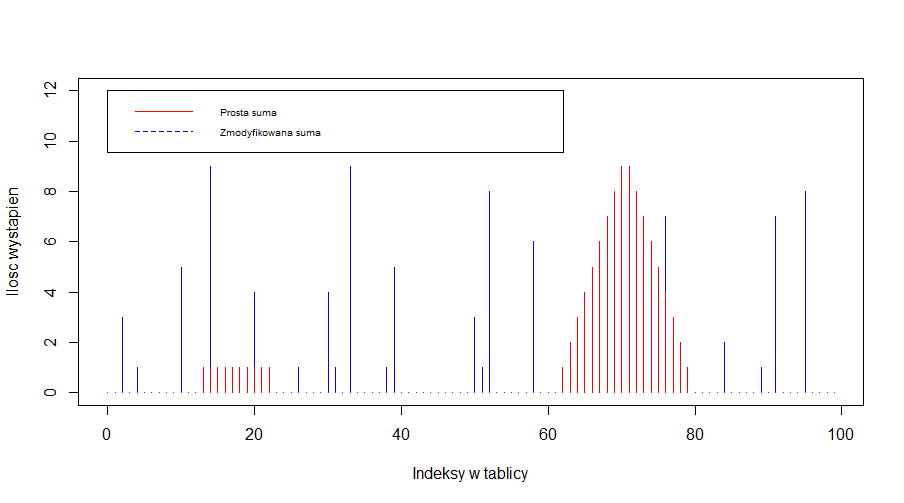
\includegraphics[width=160mm]{porownanie.png}
			\caption{Porównanie pokrycia indeksów dla funkcji haszujących.}
			\label{r1}
		\end{figure}
		
	Zajętość kluczy w tablicy znacząco się od siebie różni, ale nie jest to kryterium wpływające na ocenę funkcji haszującej.
	\clearpage
	\subsection{Zajętość miejsc}
	Pokrycie indeksów dla wcześniej wymienionych funkcji haszujących oraz tego samego zestawu kluczy przedstawiony jest w tabeli \ref{t1}.
	
	\begin{table}[!h]
		\centering		
		\caption{Porównanie pokrycia indeksów dla funkcji haszujących.}
		\begin{tabular}{|c|c|c|}
			\hline
			\textbf{Liczba wystąpień} & \textbf{Prosta suma} & \textbf{Zmodyfikowana suma} \\\hline\hline 
			0 &72 &73 \\\hline  
			1 &12 &11 \\\hline 
			2 &2&2 \\\hline 
			3 &2 &2 \\\hline 
			4 &2 &2 \\\hline 
			5 &2 &2 \\\hline 
			6 &2 &1 \\\hline 
			7 &2 &3 \\\hline 
			8 &2 &2 \\\hline 
			9 &2 &2 \\\hline 
			10 &0 &0 \\\hline 
			\ldots &0 &0 \\\hline 			
		\end{tabular} 
		\label{t1}
	\end{table} 
	
	Z tabeli \ref{t1} można wyciągnąć wniosek, że dla prostej funkcji haszującej zajętych jest tylko \texttt{28} indeksów tablicy haszującej, a dla zmodyfikowanej funkcji haszującej jest o jeden mniej --- \texttt{27}. 
\section{Podsumowanie}
Funkcja haszujaca opisana w paragrafie \ref{p1} jest porównywalnie dobra w porównaniu do prostej funkcji haszującej.

\mdfdefinestyle{eliasp}{%
	roundcorner=3pt,
	hidealllines=false,
	leftline=true,
	linewidth=0.1em
}

\section{Listingi plików}
	\subsection{Rozkład kluczy w tablicy dla funkcji haszującej z paragrafu \ref{p1}}
		\begin{mdframed}[style=eliasp]
			\lstinputlisting{czech2.csv}
		\end{mdframed}	
	\subsection{Rozkład kluczy w tablicy dla prostej funkcji haszującej}
		\begin{mdframed}[style=eliasp]
			\lstinputlisting{czech2standard.csv}
		\end{mdframed}	
	\begin{figure}[h] 		
		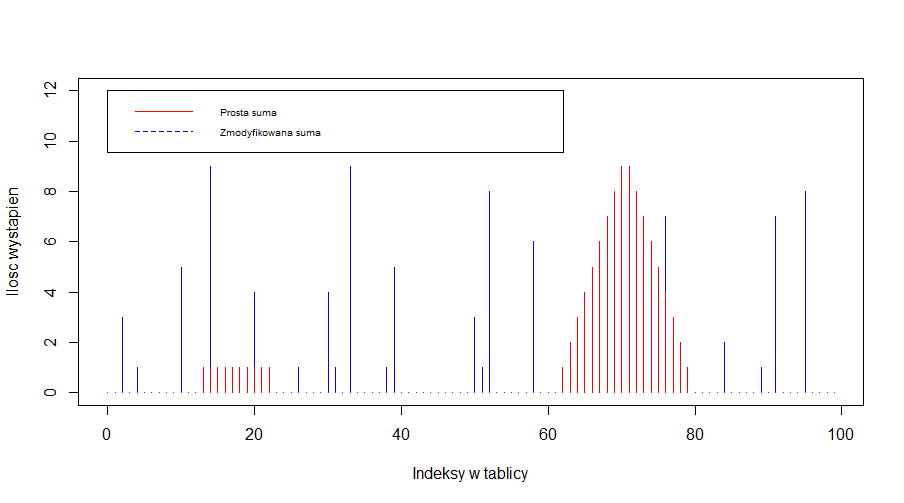
\includegraphics[angle=90]{porownanie.png}
		\label{r2}
		\caption{Porównanie pokrycia indeksów dla funkcji haszujących.}	
	\end{figure}
\section{Użyte programy}
\begin{itemize}
	\item Java - jako język programowania do generowania wyników
	\item R - język i środowisko do generowania wykresów
\end{itemize}
\end{document}